\documentclass[%
master,         % тип документа
subf,           % подключить и настроить пакет subfig для вложенной нумерации рисунков
href,           % подключить и настроить пакет hyperref
colorlinks=true % цветные гиперссылки
%,times         % шрифт Times как основной
%,fixint=false  % отключить прямые знаки интегралов
]{disser}

\usepackage[
  a4paper, mag=1000,
  left=2.5cm, right=1cm, top=2cm, bottom=2cm, headsep=0.7cm, footskip=1cm
]{geometry}
\usepackage[T2A]{fontenc}
\usepackage[utf8]{inputenc}
\usepackage[english,russian]{babel}
\usepackage{algorithm}
\usepackage{cleveref}
\usepackage{footnote}
\usepackage{totcount}
\usepackage{algpseudocode}
\ifpdf\usepackage{epstopdf}\fi

% Номера страниц снизу и по центру
\pagestyle{footcenter}
\chapterpagestyle{footcenter}

% Точка с запятой в качестве разделителя между номерами цитирований
%\setcitestyle{semicolon}

% Использовать полужирное начертание для векторов
\let\vec=\mathbf

% Включать подсекции в оглавление
\setcounter{tocdepth}{2}
\graphicspath{{../images/}}
\captionsetup[subfigure]{labelformat=parens, labelsep=space}
\bibliographystyle{gost705}
\regtotcounter{page}
\regtotcounter{figure}
\regtotcounter{table}

\newtotcounter{figuresnum}
\def\oldfigure{} \let\oldfigure=\figure
\def\figure{\stepcounter{figuresnum}\oldfigure}

%\newtotcounter{tablesnum}
%\def\oldtable{} \let\oldtable=\table
%\def\table{\stepcounter{tablesnum}\oldtable}

\begin{document}
\algnotext{EndFor}
\algnotext{EndIf}
\algnotext{EndWhile}
\newcommand*\thesubfloatfigure{\themainfigure\alph{subfloatfigure}}

\institution{\begin{figure}
	
\includegraphics[scale = 0.250]{aulogo.eps}
\end{figure}
}

% Имя лица, допускающего к защите (зав. кафедрой)

\apname{А.В. Омельченко}

\title{\bf{ДИССЕРТАЦИЯ}\\[-14pt]\textnormal{НА СОИСКАНИЕ УЧЕНОЙ СТЕПЕНИ}\\МАГИСТРА}

\topic{Анализ поверхности взаимодействия белков и поиск наиболее значительных позиций методом in silico Ala-scan \vspace{-1cm}}

% Автор
\author        {Т.С. Малыгина} % ФИО
\coursenum {010900.68} % Номер направления
\course       {Прикладные математика и физика \vspace{-1cm}}

% Научный руководитель
\sa      {П.А. Яковлев}
\sastatus{}
% Рецензент
\rev      {К. Вяткина}
\revstatus{к.ф.-м.н., с.н.с.}


% Город и год
\city{Санкт-Петербург}
\date{\number\year}
\maketitle
\pagebreak

%\input{ackn}
%\input{abstract}

% Содержание
\tableofcontents
% Введение
\intro

% Глава 1
\graphicspath{{../images/intro/}}
\chapter{Постановка задачи и обзор существующих методов}
\section{Немного о белках. Основные определения}
% - что такое белки
% - из чего состоят
% - что такое поверхность белка
% - информация о вторичной структуре 
%(мб сказать что такое вторичная структура белка?  вынести во введение или первую главу)
Зачастую являясь результатом несинонимичной замены одного нуклеотида, точечная мутация одной аминокислоты может приводить к масштабным последствиям: так, например,
\subsection{Белки как основа живой материи}
\textbf{Первичная структура} белка задается последовательностью (\textbf{цепочкой}) аминокислот:

\resizebox{0.9\textwidth}{!}{
%\input{aa3_5.tex}
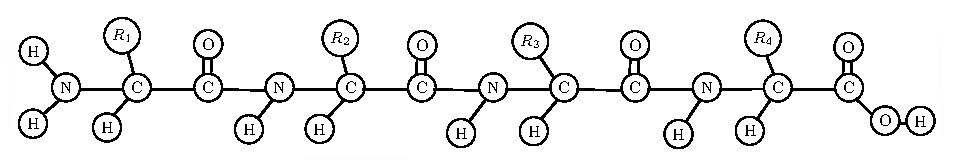
\includegraphics{aa3_1.eps}
}

\textbf{Вторичная структура} задается укладкой цепочки аминокислот в пространственные структуры, \textbf{третичная структура} - расположением этих структур в пространстве в случае, когда белок содержит только одну цепь.

Когда белок состоит из нескольких цепей, говорят о его \textbf{четвертичной структуре}.

\subsection{Белки и энергия}
С точки зрения химии, разным видам структуры соответствуют разные виды химических связей и электростатических взаимодействий.

Когда мы рассматриваем несколько цепочек в составе одного белка или несколько белков, образующих комплекс, мы говорим о \textbf{белок-белковом взаимодействии}.

\textbf{Интерфейс} такого взаимодействия -- это участки \textbf{поверхности} белков, непосредственно контактирующие между собой.

Свободная энергия связи, обозначаемая \ddG, определена как разность $\vartriangle\!G_{mut} - \vartriangle\!G_{wt}$ , где $\vartriangle\!G_{wt}$ и $\vartriangle\!G_{mut}$ -- изменения свободной энергии Гиббса для немодифицированного белка (как еще перевести wild-type?? чтоб не в лоб) и его подвергнутой точечному мутагенезу версии (alanine-mutated
protein).
\newpage
\subsection{Поверхность белка как его энергетический фронт}
\subsection{Белок-белковое взаимодействие}
Рассмотрим белок, имеющий четвертичную структуру.

\textbf{Вопрос}: можно ли изменить что-то в его структуре, чтобы образующие его цепочки были лучше сцеплены между собой?

Пусть есть комплекс из двух белков (например, имунноглобулин и эпитоп).

\textbf{Вопрос 1}: можно ли изменить что-то в его структуре, чтобы усилить связь между компонентами комплекса?

\textbf{Вопрос 2}: насколько специфична одна из компонент комплекса?  Можно ли подобрать один из белков так, чтобы комплекс был более устойчивым? Насколько заменяема каждая из компонент?

Ответить нам поможет \textbf{аланиновое сканирование} (аланиновый мутагенез).
\newpage
\section{Аланиновое сканирование}
Аланиновое сканирование (ала-скан)~\cite{alascan2001} - метод для определения аминокислот в составе белка, играющих важную роль в сохранении его функций, стабильности или формы.

Первоначальная идея метода очень проста: заменить одну из аминокислот в цепочке на любую другую и посмотреть, повлияет ли такое точечное изменение (точечный мутагенез) на энергию комплекса, приведет ли это к усилению или ослаблению взаимодействия между цепочками белков. 
\begin{center}
\resizebox{0.4\textheight}{!}{
\ttfamily
\footnotesize
\aapicture
}
\end{center}

Но как выбирать аминокислоту, на которую проводить замену? Всегда ли стоит перебирать все аминокислоты в одной и той же позиции в цепочке?

 Экспериментально было показано~\cite{alascan2001}, что достаточно заменить аминокислоту на аланин, чтобы понять, является ли она энергетически значимой при оценке взаимодействия цепочек, или нет. А затем, если изменение энергии комплекса \ddG  оказывается существенным, перебрать все оставшиеся аминокислоты в данной позиции и определить, какая замена является экстремальной.

\begin{wrapfigure}{RT}{0.3\textwidth}
\resizebox{0.3\textwidth}{!}{
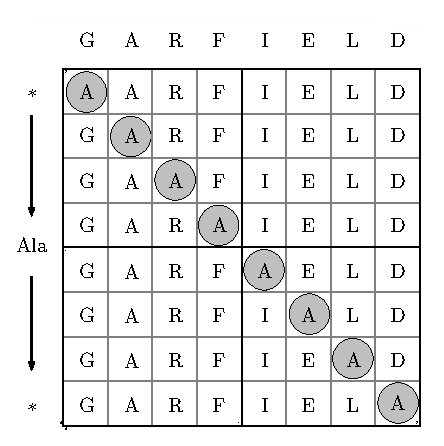
\includegraphics{ala_scan.eps}
}
\end{wrapfigure}
\newpage
\subsection{Аланиновое сканирование in vitro/in vivo}
Первоначально аланиновое сканирование появилось как лабораторный, химический метод (in vitro/in vivo), с вытекающими отсюда недостатками:
\begin{itemize}
\item Большое пространство поиска: для того, чтобы определить энергетически значимые аминокислоты, требовалось проверить все.
\item Сложность синтеза библиотек: необходим индивидуальный подход, сложность с разделением образцов с мутациями, сложность получения образцов с точечной мутацией в нужной позиции.
\item как следствие, высокая стоимость.
\end{itemize}

Впоследствии появились базы данных с результатами аланинового сканирования ~\cite{asedb2001, bid2003}, но они фрагментированы, не всегда полны, разнородны. Кроме того, данных в них не так много - в силу приведенных выше недостатков проведения точечного мутагенеза в лаборатории.

Например, если Protein Data Bank содержит информацию о большом количестве структур, с примерно одним и тем же форматом данных, то asedb представляет собой базу данных mysql и содержит информацию о 101 структуре, а bid доступен в виде набора wiki-страниц с информацией о конкретных белках или парах взаимодействующих цепочек.
%уточнить цифру
 \newpage
\subsection{Аланиновое сканирование in silico: решаемые задачи и границы применимости}
\todo{написать про метод, протоколы, используемые функции, что такое дельта-дельта G}

\todo{сказать, что в данной работе используется протокол из rosetta (мб привести картинку про реальную ddG и in silico функцию изменения энергии), сцепленность цепочек оценивается в смысле изменения энергии, применяемый в протоколе метод монте-карло лежит за пределами работы (кроме того, является относительно хорошо изученным, в ходе работы никакие модификации в сам метод или функцию оценки ddG не вносились), поэтому не приводится. }

\newpage
\section{Стандартные методы выбора аминокислот для аланинового сканирования in silico}

Как правило, при компьютерном моделировании аланинового сканирования применяют предварительную фильтрацию аминокислот, после которой проводится сканирование. Для фильтрации используются два основных метода~\cite{hotspots2012rev}:
\begin{itemize}
\item отсечка по расстоянию ~\cite{kortemme2004}: мутации подвергаются только те аминокислоты, которые расположены вблизи области взаимодействия пары белков;

\item выбор по гомологии: аминокислоты выбираются исходя из имеющихся экспериментальных результатов аланинового сканирования, проводившихся на близких (в эволюционном смысле) последовательностях.
\end{itemize}

Оценим эффективость этих подходов.

\subsection{Использование отсечки по расстоянию}

\begin{itemize}
\item Аланиновому сканированию подвергаются аминокислоты цепочки, образующей комплекс совместно с другой цепочкой, содержащие атомы, удаленные от каких-либо атомов цепочки, также участвующей в образовании комплекса, на расстояние, не превышающей некоторой фиксированной величины

\item В качестве порогового значения расстояния используются, например, величины 4, 5, 8 \AA{}

\item в Rosetta Alascan Protocol~\cite{kortemme2004} используется усложнение: дополнительно рассматриваются аминокислоты, $\beta$-углерод которых после формирования комплекса в шаре определенного фиксированного радиуса содержит существенно больше атомов $\beta$-углерода, чем содержал до этого.
\end{itemize}
\newpage
Эксперимент
\begin{itemize}
\item Рассмотрим базу данных с информацией о результатах эспериментов по аланиновому сканированию белков ASEdb~\cite{asedb2001}.
\item Найдем объекты с корректными ссылками на записи в Protein Data Bank ~\cite{rcsb}.
\item Среди всех таких объектов, найдем те, в которых есть аминокислоты, мутация которых приводит к существенному изменению свободной энергии комплекса ($\geq 1$ ккал/моль)
\item Посмотрим, всегда ли они удалены от интерфейса в пределах стандартно используемой отсечки (в качестве примера возьмем расстояние, не превышающее 8 \AA{}).
\end{itemize}

\resizebox{0.8\textwidth}{!}{
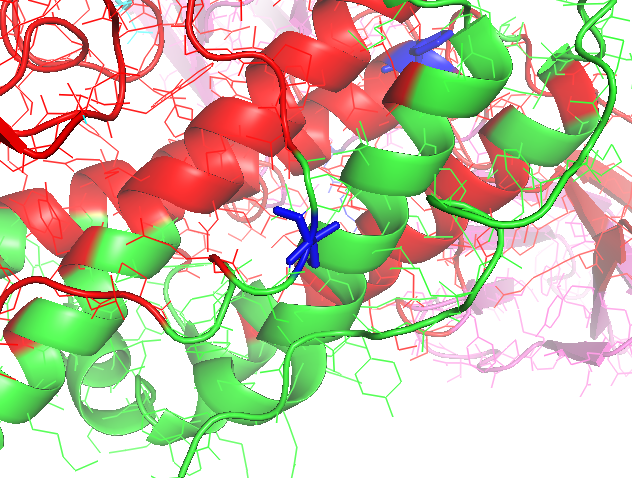
\includegraphics{image7.png}
}

\newpage
\subsection{Поиск по гомологии}
Для эффективного поиска по гомологии необходимо иметь базу близких (ортологичных) структур, точную и содержащую всю информацию по результатам аланинового сканирования.

Метод должен учитывать как данные о последовательности аминокислот в белках, так и каким-либо образом эксплуатировать пространственную структуру. В качестве примеров методов, учитывающих и то, и другое, можно привести ~\cite{hhm_svm}.

Проводятся попытки классификации участков, 
%здесь можно ссылку на диссертацию студентки Фришмана

% Глава 2
\graphicspath{{../images/algorithm/}}
\chapter{Описание разработанного метода}

\section{Биологическое обоснование}
Как видно из предыдущей главы,  в настоящий момент при выборе аминокислот, подвергаемых точечному аланиновому мутагенезу, не проводится какой-либо сложный анализ.

\todo{спорное утверждение все-таки, немного противоречит статье про петли, может, лучше как-то помягче сформулировать?}

% О-кольца
% фрагменты петель
% гидрофобность
% карманы

%\newpage
\subsection{Гидрофобность}
Широко известна и подтверждена гипотеза о том, что фолдинг белков происходит под влиянием свойств аминокислот: гидрофобные аминокислоты стремятся оказаться внутри, поскольку стараются избегать воду, которая находится снаружи от сворачивающейся молекулы \cite{hydrophoby}.

Похожим образом интерфейс взаимодействия цепочек, связь между ними образуется за счет гидрофобных взаимодействий: в область связывания попадают в первую очередь гидрофобные аминокислоты, находящиеся на поверхности цепочки белка.

%\newpage
\subsection{Карманы}
A complemented pocket is a concave surface
region on one protein chain that is filled by its
binding partner, representing a tight fit.
\cite{pockets2004}
%\newpage
\subsection{Петли}
Попытка обобщить понятие энергетически горячего аминокислотного остатка до регионов проводится в работе~\cite{loops2014}. В ней вводится понятие ,,горячей петли'' -- такого короткого (до 10 аминокислот) фрагмента  цепочки белка, содержащей более 2 энергетически значимых аминокислотных остатков. В упомянутой статье проводится анализ таких петель по данным ASEdb~\cite{asedb2001} и попытка каким-то образом сгруппировать их и сделать выводы о том, какие аминокислоты чаще встречаются в таких ,,горячих петлях''.

Идея о возможности обобщения основана на понятии о гибкости петель, их способности существенно менять положение в пространстве в зависимости от поворота образующих их аминокислот.

%о которой известно, что она моЧто там происходит: взята ASEdb, рассмотрены короткие фрагменты петель, содержащие энергетически горячие аминокислоты и приведена их какая-то классификация.
\subsection{Поиск по гомологии}
Уместно учесть информацию об энергетически значимых аминокислотах в тех ситуациях, когда одна из рассматриваемых цепочек комплекса близка (в эволюционном смысле) к цепочке комплекса, для которого результаты аланинового сканирования известны, а парная цепочка или лиганд, с которой (которым) оценивается взаимодействие, совпадает.

Такое расширение алгоритма может помочь учитывать ситуации, когда энергетический вклад аминокислоты меняется (в большую или меньшую сторону) за счет не мутации, а поворота, происходящего под воздействием изменившегося положения аминокислот, принадлежащих удаленному от интерфейса фрагменту цепочки, сдвинувшемуся в результате точечной модификации (визуально это может выглядеть, например, как каскад петель - см. рисунок ??). 
%\newpage
\section{Входные данные}

На входе PDB~\cite{pdb}, в каком виде данные. единицы измерения, точность
%(полстраницы, возможно, с картинкой)
%\vspace{10cm}

\resizebox{0.8\textwidth}{!}{
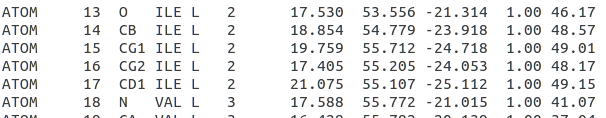
\includegraphics{atom_in_pdb.png}
}

PDB файл ~\cite{pdb} содержит информацию о белке, сгруппированную по следующим признакам: 
\begin{enumerate}
\item пространственное положение атомов аминокислот (секция ATOM):
включает информацию о координатах каждого из атомов, образующих аминокислоты, в свою очередь образующих цепочки белка или белков, вид атома, другие важные характеристики. Координаты упорядочены по положению аминокислот в цепочке.

\item информацию о вторичной структуре цепочек (секции helix, sheet)
\end{enumerate}


%\newpage
\section{Выбор протяженных регионов}
Для того, чтобы выбрать протяженные регионы для аланинового сканирования, построим итеративный алгоритм.

Включим в состав множества протяженных регионов, содержащих ,,энергетически горячие аминокислотные остатки'', следующее:
\begin{itemize}
\item аминокислоты, образующие ,,интерфейс'' взаимодействия с парной цепочкой или белком (с использованием отсечки по расстоянию от второй цепочки)
\item аминокислоты, образующие поверхность ,,карманов'', находящихся в области взаимодействия пары белков
\item не-гидрофобные аминокислоты, являющиеся соседними по отношению к аминокислотам, образующим интерфейс
\item если интерфейс взаимодействия образован петлями, то добавим все аминокислоты, образующие петли 
\end{itemize}


%\newpage
\subsection{Формализация задачи}
%\begin{frame}{Formal definitions - I}
%\begin{itemize}
%\item Protein molecule - a set of spheres S. Each sphere $s \in S,\,s=s(c_s, r_s)$ has center point $c_s$ and radius $r_s$, ,,atom'' corresponds to sphere.
%\item the Euclidean distance $D(x,\,s)$ 
%of a point $x$ from the surface of a sphere $s$:
%$$
%D(x,\,s) = || x - c_s || - r_s
%$$
%\item The minimal distance from the point x to the nearest sphere (atom) is given by the function r (x):
%$$
%r(x) = \min \{D(x,s) | s \in S \}
%$$
%\end{itemize}
%\end{frame}

\subsection{Маскировка аминокислот}
В качестве предварительной обработки добавим возможность маскировки аминокислот -- исключения из рассмотрения тех фрагментов цепочек, аминокислоты на которых нам не интересны или которые изменять не желательно. В качестве примера возьмем случай, когда мы хотим усилить сцепленность между легкой и тяжелой цепями антитела, но при этом не хотим никак повлиять на его специфичность -- в этом случае уместно исключить из рассмотрения CDR-регионы.

%\todo{или идея в том, что мы не рассматриваем CDR потому что они гипервариабельные, и изменить одну амк на них технически нереально?}
%Исходя
\subsection{Триангуляция Делоне}
%\newpage
\subsection{Построение графа}
\begin{itemize}
\item Рассматриваем одновременно 2 цепочки, образующие белковый комплекс.
\item Начнем с построения выпуклой оболочки и триангуляции Делоне для каждой из них, будем искать протяженные регионы с энергетически горячими аминокислотными остатками  на одной из них. Строить будем по центрам атомов, формирующих аминокислоты цепочки.
\item Выберем все треугольники выпуклой оболочки, в которых хотя бы одна вершина удалена от некоторых атомов второй цепочки не далее, чем на выбранное (фиксированное) значение отсечки.
\end{itemize}


\begin{itemize}
\item Берется структура в PDB.
\item Центры атомов рассматриваются как точки. По ним строится триангуляция Делоне (с помощью scipy.delaunay - обертки над алгоритмом qhull).
\item Берется невзвешенная триангуляция -- по тем же соображениям, по которым она используется в CAVER (эвристика)\cite{caver2007}.
\end{itemize}
Я сопоставляю графу триангуляцию по тому же принципу, как в статье по CAVER:

\begin{center}
\resizebox{!}{0.3\textheight}{
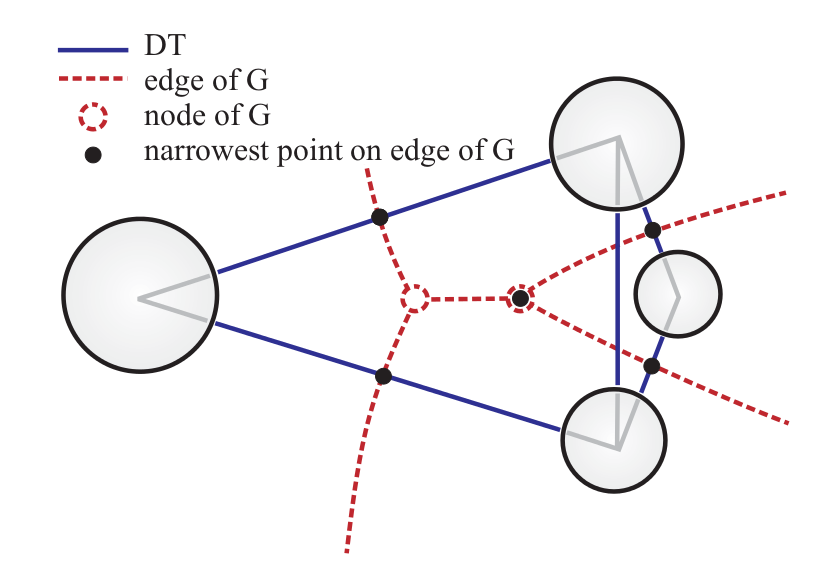
\includegraphics{image4_caver.png}
}

[Computation of tunnels in protein molecules using
Delaunay triangulation, P.Medek, et al., 2007]
\end{center}

Треугольники триангуляции -- вершины графа, ребра графа -- общие стороны треугольников (с ограничением снизу на длину).

Дополнительно используется такой же граф по треугольникам выпуклой оболочки (без ограничения снизу на длину стороны, просто по смежным по стороне треугольникам).

Выбирается начальное множество треугольников выпуклой оболочки. Сейчас берутся треугольники, вершины которых недалеко (в смысле отсечки по расстоянию) от второго белка.

%\newpage
\subsection{Псевдо-интерфейс}
\todo{вспомнить, что я хотела сказать таким заголовком}
\begin{itemize}
\item определяем множество треугольников выпуклой оболочки, для которых хотя бы одна вершина удалена от центров атомов второй цепочки не больше, чем на выбранное значение отсечки
\item Далее расширяем интерфейс
\begin{itemize}
\item шаг 1: добавляем к интерфейсу все треугольники выпуклой оболочки, содержащие атомы аминокислот, которые уже туда попали
\item шаг 2: продлеваем регион до границы гидрофобности
\item шаг 3: продлеваем регион за границы гидрофобности на 1 аминокислоту.
\end{itemize}
\end{itemize}


В результате у нас есть одна или нескольких протяженных связных областей выпуклой оболочки, по которым можно восстановить аминокислоты.
%\newpage
\subsection{Поиск карманов}
\todo{переписать}
Поиск карманов, каналов и полостей в макромолекулах является хорошо изученной задачей \cite{alpha_shapes1995, alpha_shapes1998, caver, ppi_kim2006}.  

\begin{itemize}
\item Начинаем с множества отобранных треугольников выпуклой оболочки (черным цветом)
\item Ищем в ширину с ограничениями
\item Ходим только по тем треугольникам, для которых ближайший треугольник выпуклой оболочки -- один из отобранных треугольников выпуклой оболочки, а не какой-либо из других треугольников выпуклой оболочки.
\item Ближайший треугольник == в смысле расстояния до ближайшей из вершин он ближе, чем другие треугольники выпуклой оболочки
\end{itemize}
\cite{alpha_shapes1995, alpha_shapes1998}
%\newpage
\subsection{Расширение интерфейса. Добавление петель}

Перед добавлением петель треугольники триангуляции преобразуются в фрагменты последовательности аминокислот, продлеваем их, используя информацию о вторичной структуре.



Сейчас вторичная структура определяются на основе вывода DSSP \footnote{используется обертка к DSSP в составе biopython}.

Берутся непрерывные фрагменты структуры, которые не определяются как $\alpha$-спирали или $\beta$-листы, выбираю среди них те, в которые попадает какая-либо аминокислота, добавляются к выделяемому контуру.

%\todo{\item Я беру непрерывные фрагменты структуры, которые не определяются как альфа-спирали или бета-листы, выбираю среди них те, в которые попадает какая-либо аминокислота, ну и добавляю их к выделяемому контуру - технической сложности никакой.}




%\begin{itemize}


%\todo{\item вариантов 2: либо не добавлять петли целиком, вместо этого добавлять только такие фрагменты (в статье они приведены), либо как-то их отмечать на выделенных петлях + отмечать на удаленных петлях, которые в выделенный регион не попали.}

% \todo{\item про HMM думаю, напишу через пару дней.}

% \todo{\item вообще если получится, я разберусь как считать взвешенную триангуляцию Делоне и с помощью нее искать карманы.}


%\end{itemize}

% Глава 2
\chapter{����������������� ����������}

\section{��������� � ������� �������������}

\subsection{������������ ��������������� ������}




\subsection{�������� ������}



% Заключение
\conclusion
В данной работе был построен алгоритм поиска протяженных регионов, определяющих специфичность белка по отношению к белковому комплексу, основанный на общих представлениях об энергетически значимых аминокислотах, которые оказывают существенный вклад в функцию, стабильность или форму белка, и тем самым формируют такие регионы. 

Было проведено тестирование алгоритма на наборе данных Kortemme \& Baker, показано, что в такие регионы попадают все (или почти все) энергетически значимые аминокислоты, которые были определены экспериментально.

Тем не менее, получаемый таким образом регион, определяющий специфичность -- достаточно обширен; это приводит к низкой  точности такого метода. Низкую точность можно объяснить следующими причинами:
\begin{itemize}
\item задача предсказания энергетически значимых аминокислот является труднорешаемой и трудноформализуемой, на текущий момент нет  инструментов, позволяющих предсказывать энергетически значимые аминокислоты с высокой точностью; 
\item хотя приведенный алгоритм позволяет выявить регионы, определяющие специфичность, задача определения энергетически значимых аминокислот на них  осложняется тем, что энергетическая значимость аминокислоты может быть получена в том числе за счет изменения положения боковых цепей соседних с ней аминокислот, то есть она зависима от окружения.
\end{itemize}

Полученный алгоритм может быть использован  для выбора аминокислот и проведения дальнейшего аланинового сканирования in silico. Он реализован на языке python, с применением библиотек SciPy\cite{scipy} и NumPy\cite{numpy}.

Кроме того, написан плагин для приложения PyMOL~\cite{pymol}, визуализирующий регион, определяющий специфичность, для выбранной структуры.




% Список литературы

\bibliography{thesis}

\end{document}
